	\begin{Huge}
				Bioinformatik
			\end{Huge}
			\begin{exampleblock}{\textcolor{white}{Was ist der Studiengang?}}
				Grob gesagt die Schnittstelle zwischen dem Chemiker im Labor und der Datenverarbeitung am Rechner. Mögliche Schwerpunkte gehen in Richtung automatisierte Verarbeitung von DNA-Daten, Drug Design, Krebsforschung etc.
				Das Studium beinhaltet neben der klassischen Informatik Inhalte aus Molekularbiologie, Neurobiologie, Biochemie und Chemie. Ein Schwerpunktfach gibt es nicht. Danach kann das Studium mit einem Master (4 Semester Regelstudienzeit) weitergeführt werden.
			\end{exampleblock}
			\begin{block}{Welcher Teil macht wie viel im Studium aus?}
				\begin{figure}[h!]
						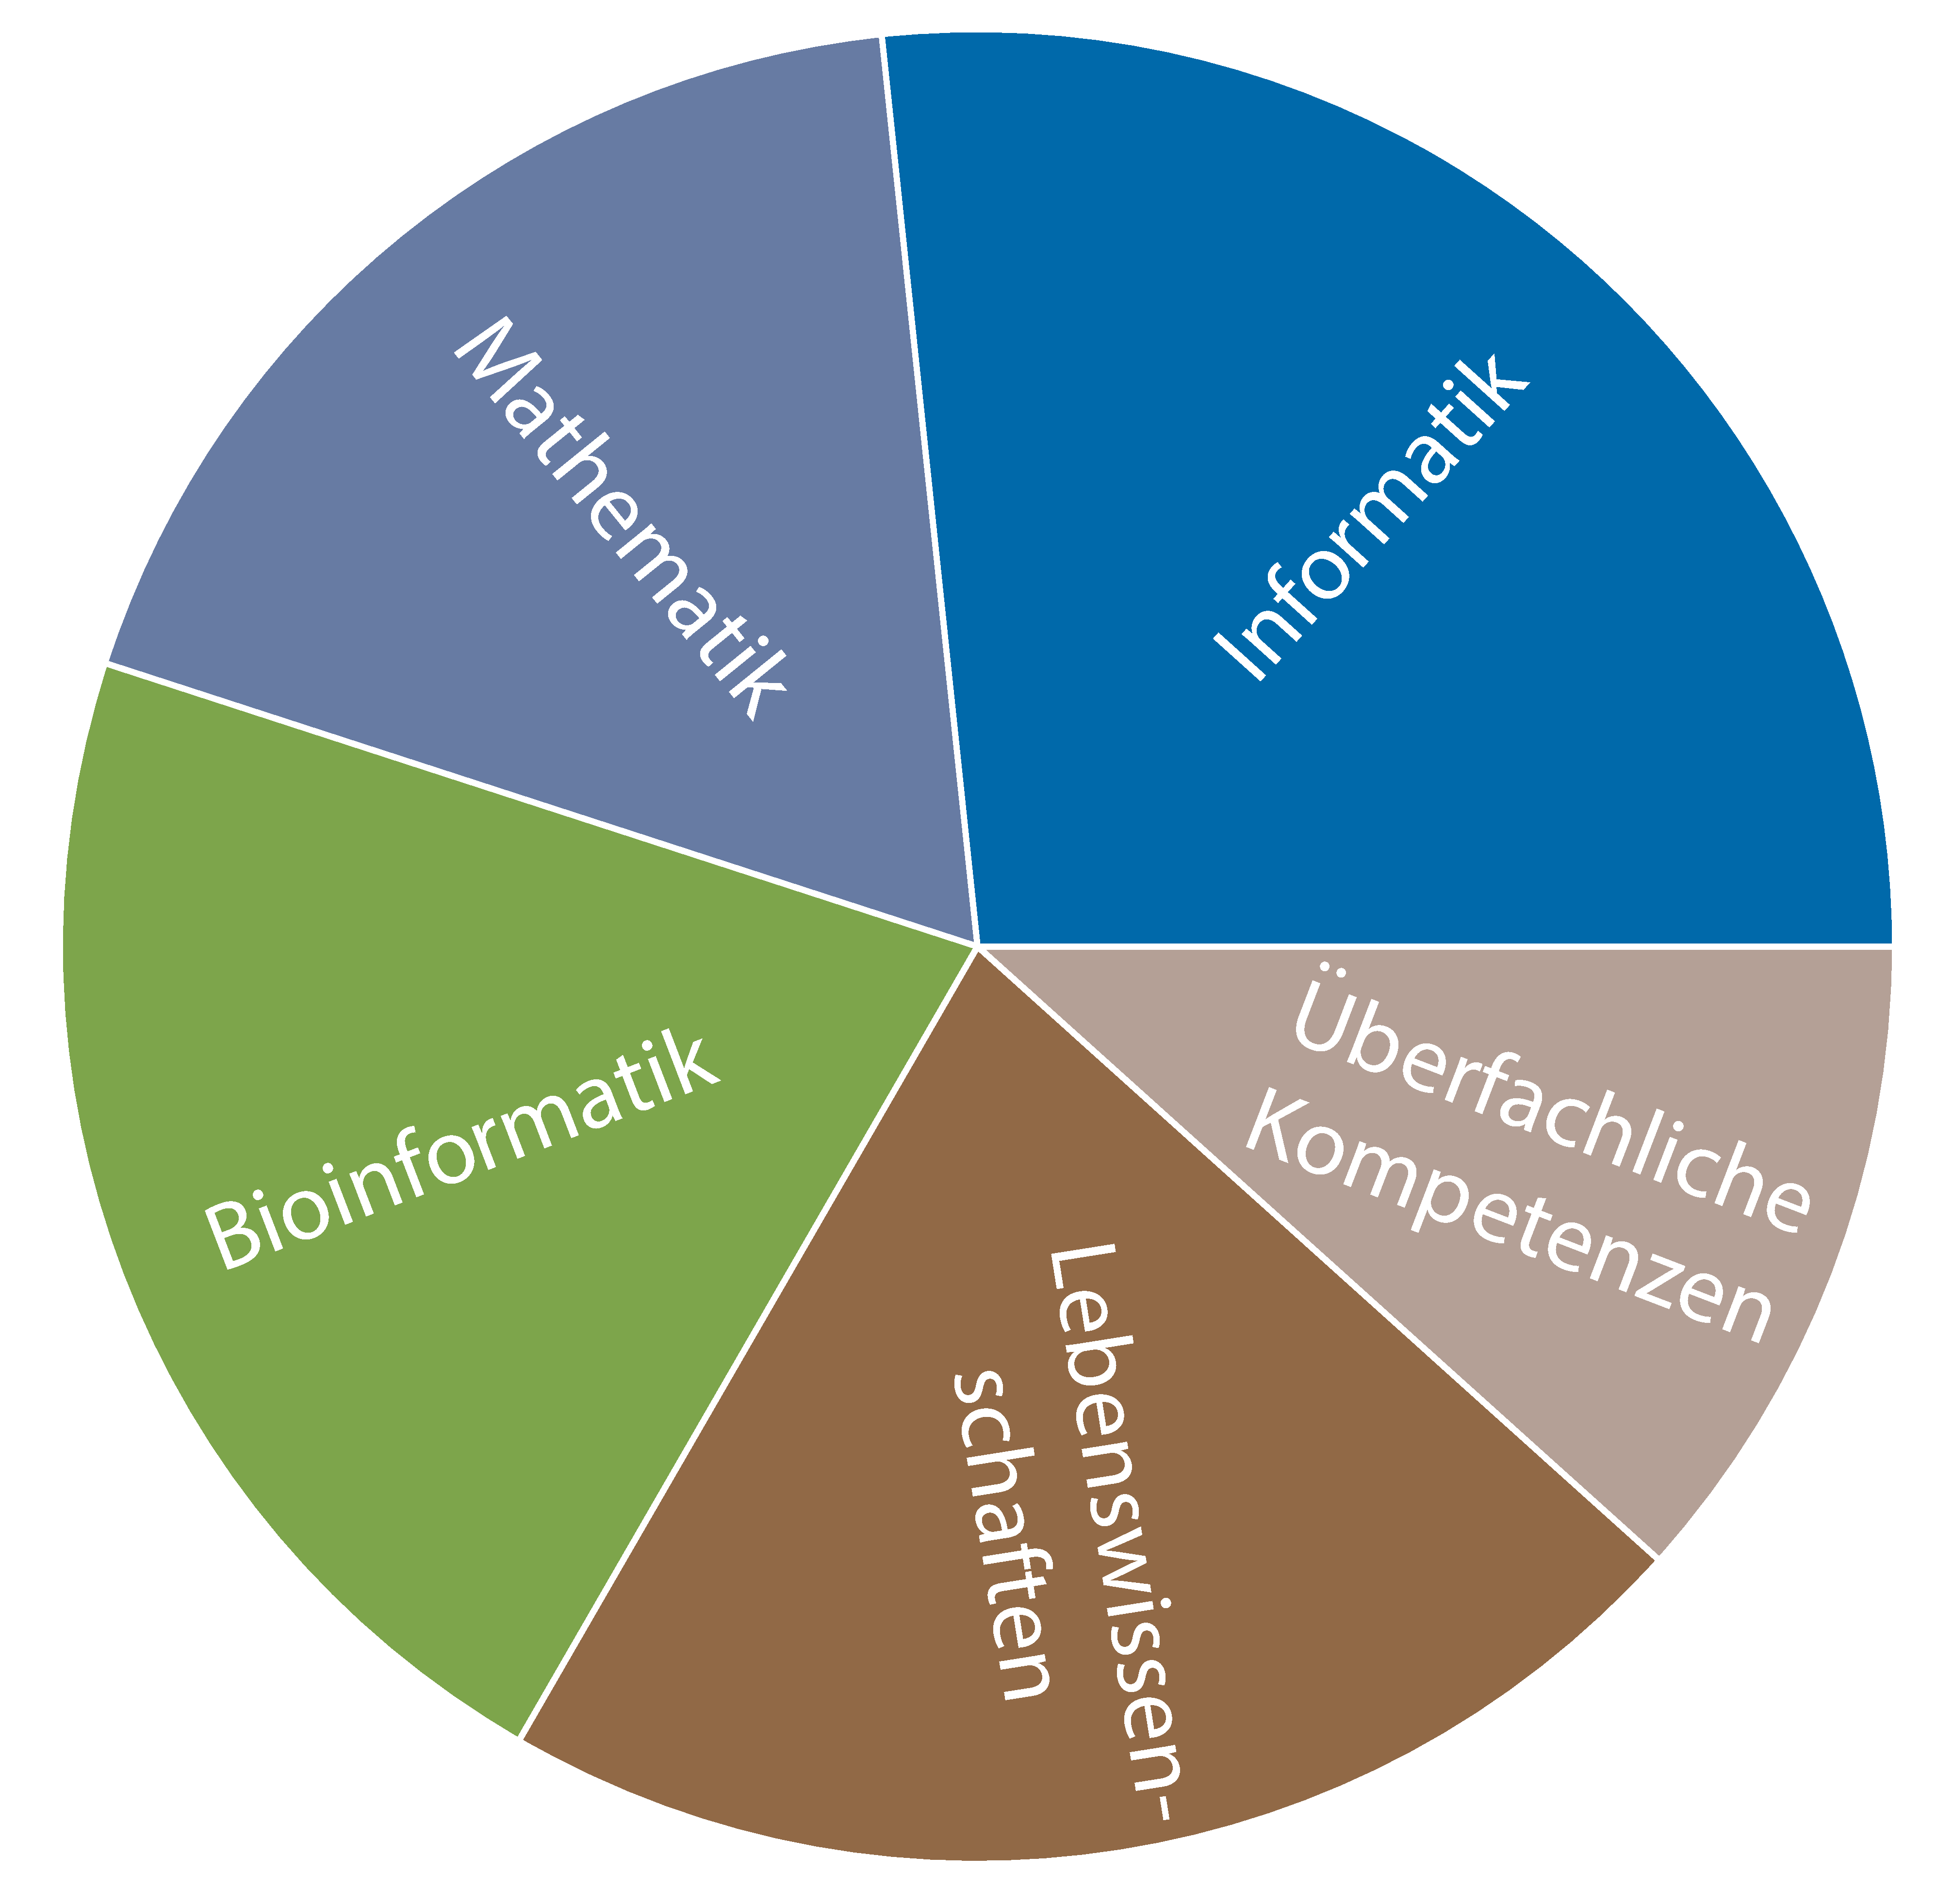
\includegraphics[width=0.4\textwidth]{charts/bioinformatik-Piechart.pdf}
					\caption{Verteilung der Themenbereiche über das komplette Studium}
				\end{figure}
			\end{block}
		\begin{block}{Was macht man in welchem Semester?}
			\begin{figure}[h!]
					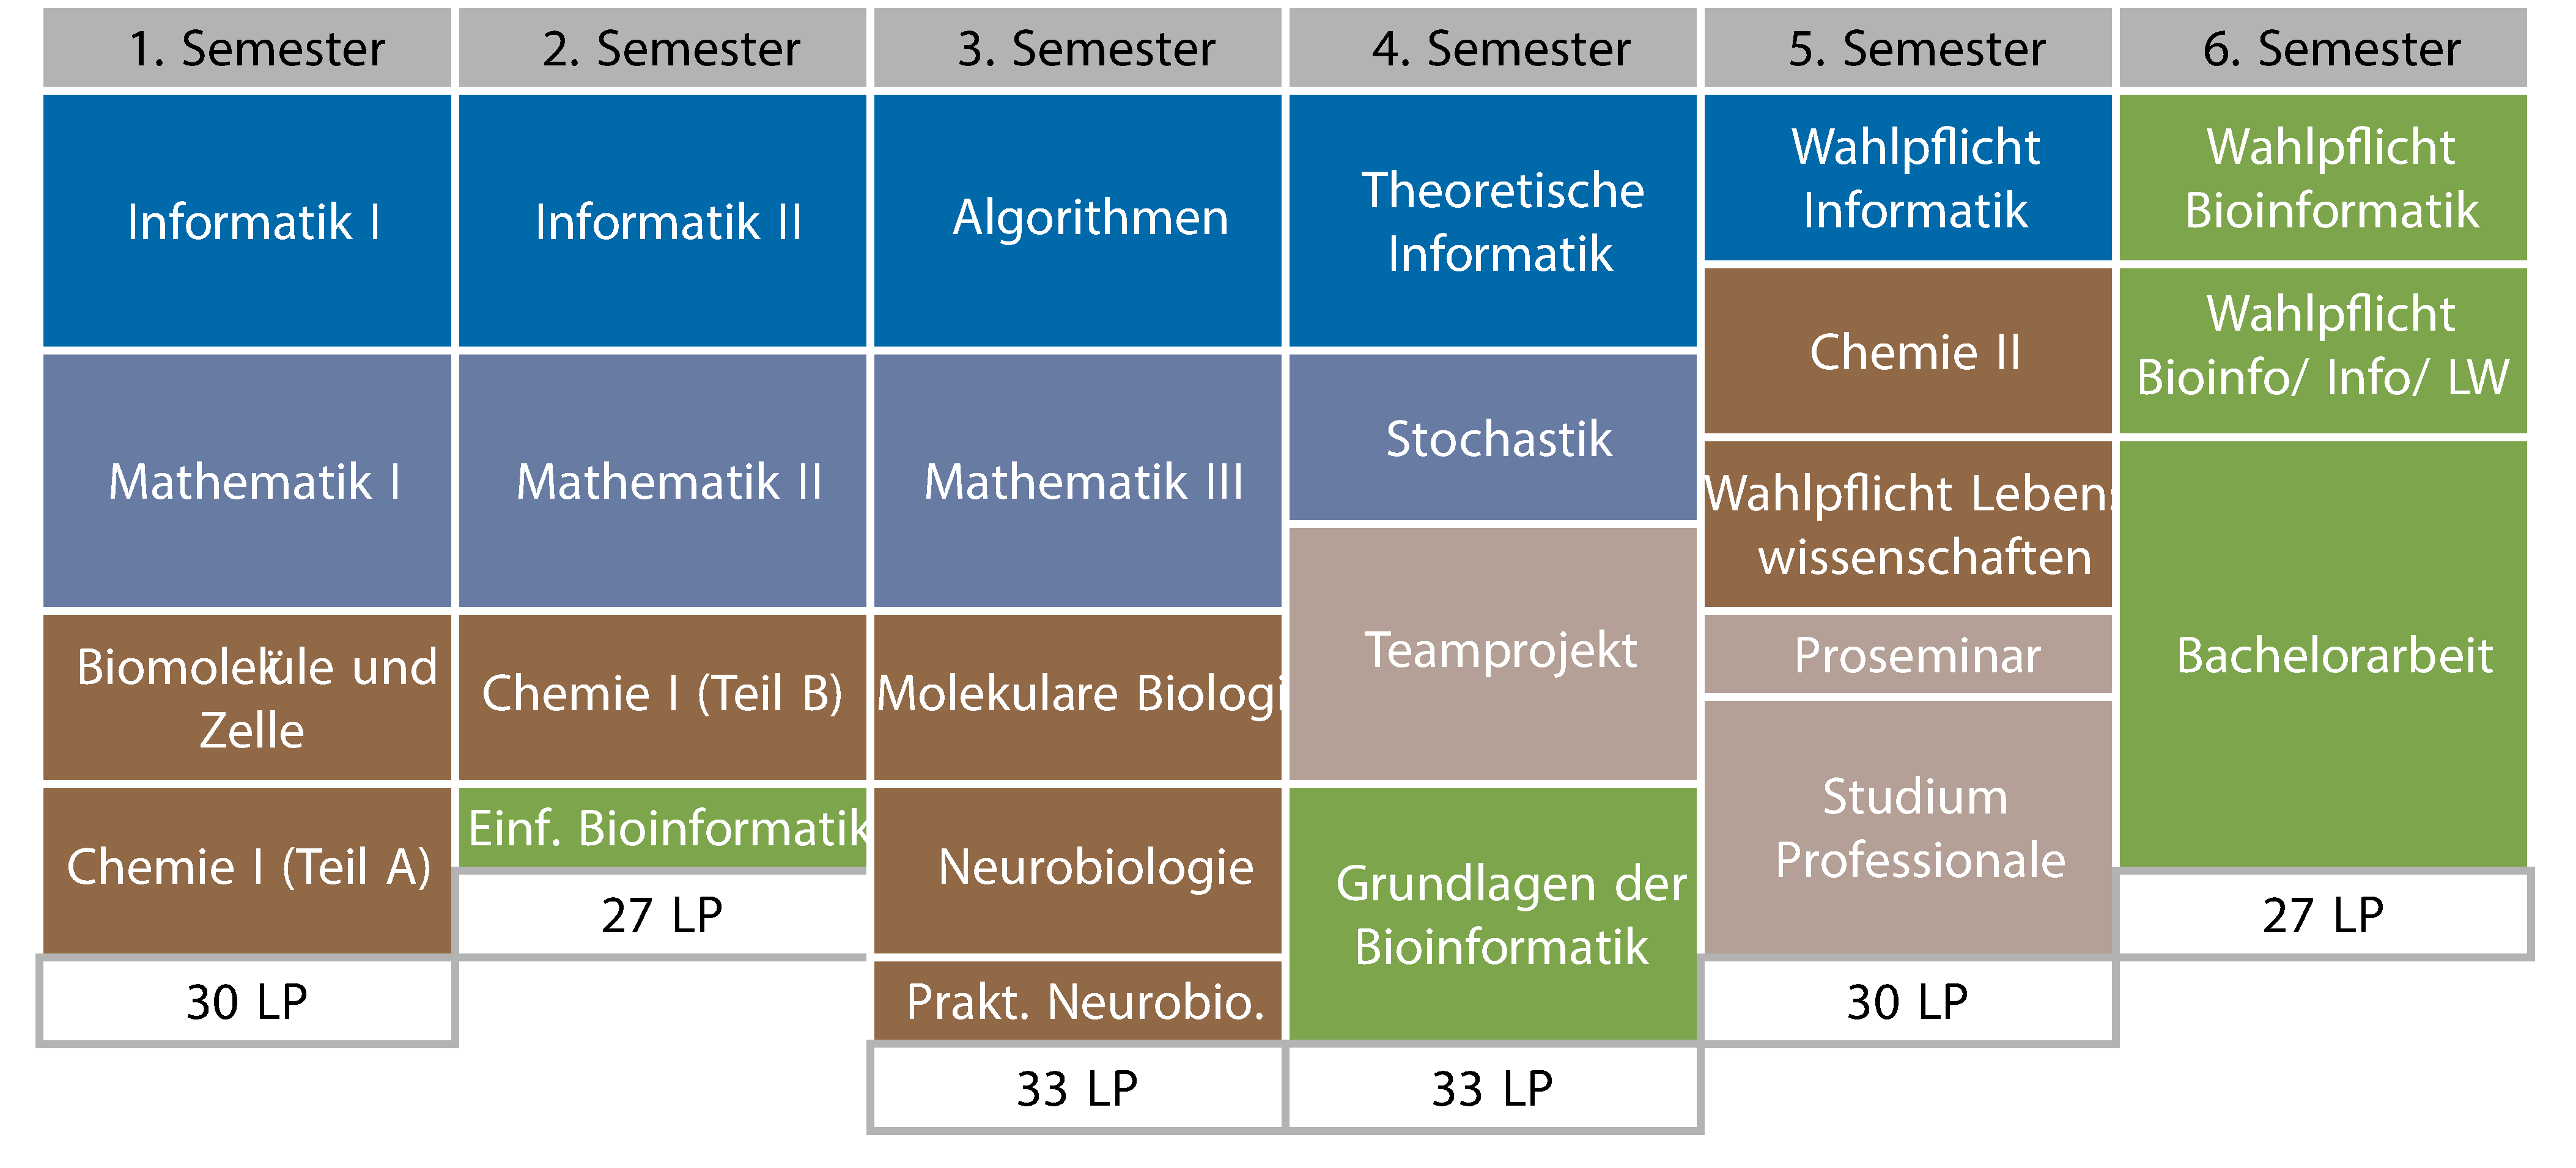
\includegraphics[width=\textwidth]{charts/bioinformatik-Studienplan_abWS18.pdf}
			\end{figure}
		Das 1. Semester ist nach Plan ein Wintersemester. Wenn du dein Studium zum Sommersemester beginnen möchtest, beginnst du im Plan bei Semester 2 und machst dann Semester 1. 
		Dieser Verlauf ist unabhängig vom Studienbeginn nur ein Vorschlag und kein bindender Studienplan. Es empfiehlt sich jedoch, den Plan einzuhalten, wenn man in Regelstudienzeit studieren möchte.
		\end{block}
	\vfill
	\begin{flushright}
		
\includegraphics[width=0.4\textwidth]{fsilogo.pdf}
	\end{flushright}